\capitulo{3}{Conceptos teóricos}

Este capítulo tiene como objetivo exponer de manera detallada los conceptos teóricos que consolidan las bases del proyecto. Para facilitar la comprensión de los numerosos conceptos que han hecho su aparición en el desarrollo se ha tomado la decisión de agrupar estos en 3 secciones. Primeramente, se desarrollarán aquellos \hyperref[sec:gestionproyectos]{conceptos relacionados con la organización y gestión de proyectos}. Seguidamente, se expondrán \hyperref[sec:conceptosextraccionprocesamiento]{nociones relativas a la extracción y el preprocesamiento de los datos}. Finalmente, se presentarán aquellos \hyperref[sec:procesamientodatos]{conceptos en lo referente a los modelos de procesamiento del lenguaje natural (PLN)}.

\section{Conceptos teóricos relativos a la gestión de proyectos} \label{sec:conceptosgestionproyectos}

Uno de los principales conceptos con los que se presentó la idea original de proyecto radicaba en trabajar con la idea de la \hyperref[sec:gestionproyectos]{gestión de proyectos} aplicando técnicas de \textbf{Inteligencia Artificial (IA)}. La gestión de proyectos es una disciplina de la administración de empresas encargada de la aplicación de metodologías de planificación, organización, motivación y control de recursos con el objetivo de obtener un resultado único.

Como podemos deducir de la anterior definición, la gestión de proyectos está compuesta por un gran número de disciplinas que interaccionan entre sí para conducir un proyecto a un claro objetivo propuesto. El éxito de un proyecto se computa recurriendo al estudio del cumplimiento de los requisitos de este, así como las relaciones entre el tiempo, el coste y el alcance de este.

De acuerdo con el informe <<\emph{CHAOS 2020: Beyond Infinity Overview}>> \cite{ct:portman_project_success} a fecha de enero de 2021 tan solo un \textbf{31\%} de los proyectos resultan exitosos. Estos datos se presentan frente a un \textbf{50\%} que se presentan como proyectos que aun habiendo cumplido su objetivo no lograron efectuarlo respetando las restricciones inicialmente establecidas.

\subsection{Gestión de Proyectos (\emph{Project Management})} \label{sec:gestionproyectos}

Uno de los principales desafíos a los que se enfrentan los proyectos se encuentra en el proceso de planificación, gestión y seguimiento de las tareas de manera que se cumpla con los requisitos y objetivos propuestos.  \cite{ct:universal_knowledge_management}

La gestión de tareas consiste en el proceso de llevar a cabo el seguimiento de una tarea a lo largo de su ciclo de vida. Este proceso se compone de compone de una serie de fases de planificación, pruebas, \hyperref[sec:seguimientoincidencias]{seguimiento} (tracking) y generación de informes. El objetivo de la gestión de tareas es lograr que cada tarea alcance su objetivo cumpliendo con los requisitos establecidos para cada tarea individual, así como lograr establecer una comunicación entre los responsables de llevar a cabo cada tarea de manera que se consigan completar los objetivos globales.

\subsection{Seguimiento de Incidencias (\emph{Issue Tracking})} \label{sec:seguimientoincidencias}

El seguimiento de incidencias consiste en la aplicación de una serie de metodologías cuya finalidad es cumplir con la planificación inicial establecida para un proyecto manteniendo un control sobre las tareas que lo componen.

La importancia del \emph{issue tracking} recae en que los problemas que se generan en una tarea repercuten en la planificación de tareas posteriores, y en última instancia en la planificación general del proyecto, es por ello por lo que es de vital importancia localizar agilizar localización de las dificultades en el desarrollo de las tareas para que estas puedan ser solventadas con la mayor brevedad y de la manera más eficiente posible.

Para facilitar el seguimiento de un proyecto se plantea el uso de herramientas conocidas como \emph{project trackers}. Este tipo de software permite planificar el desarrollo de un proyecto estableciendo metas parciales, creando objetivos medibles que se ajusten los requisitos de manera realista, llevando un registro de los recursos o personal implicado en cada etapa o tarea del proyecto, designando periodos de reunión que fortalezcan la comunicación entre los diferentes participantes del proyecto compartiendo avances y propuestas, y estableciendo márgenes de maniobra con el objetivo de mitigar los posibles efectos de los problemas que aparezcan a lo largo de su desarrollo.

\subsection{Plataformas (\emph{GitHub})} \label{sec:plataformas}

Existen numerosas plataformas surgidas en base a la necesidad de gestionar el desarrollo de un proyecto. Por lo general, estas plataformas ofrecen soluciones que permiten almacenar y llevar un control de versiones del proyecto, y a su vez ofrecer sistemas de gestión y seguimiento de las tareas. La ventaja de esta unificación supone el poder mantener en una misma situación los detalles de los cambios, vincularlos a las incidencias y mantener las discusiones sobre su desarrollo e implementación en los comentarios de la tarea.

En el desarrollo de nuestra aplicación hemos centrado los esfuerzos en aplicar el proceso de extracción y experimentación sobre proyectos de la plataforma \emph{GitHub}. La motivación principal detrás de escoger esta plataforma, frente a sus principales alternativas \emph{GitLab} y \emph{BitBucket}, es el número de proyectos que se desarrollan a través de \emph{GitHub}.

En las siguientes secciones se van a presentar brevemente los tres elementos principales de \emph{GitHub} en los que se ha centrado la atención del proyecto: \hyperref[sec:repositorio]{los repositorios}, \hyperref[sec:incidencia]{las incidencias}, y \hyperref[sec:etiqueta]{las etiquetas}.

\subsubsection{Repositorio} \label{sec:repositorio}

Un repositorio \cite{ct:github_repository} es el concepto principal alrededor del que se construye la plataforma \emph{GitHub}. Cada repositorio representa el desarrollo de un proyecto, generalmente software. Estos repositorios permiten como funcionalidad principal la gestión y el almacenamiento de su contenido a través de un sistema control de versiones basado en la tecnología \emph{Git}. Este planteamiento permite a los participantes del proyecto poder trabajar de manera simultánea en distintas tareas y a su vez la posibilidad mantener el desarrollo siempre actualizado con los últimos cambios disponibles.

Entendiendo los repositorios como instancias de alto nivel dentro de la plataforma, estos a su vez están compuestos por multitud de entidades como son los propios ficheros que componen el proyecto, el historial de versiones de estos, las incidencias, las peticiones de cambios o los hitos. En este trabajo nos centraremos en aquella información relacionada de manera estricta con las incidencias.

\subsubsection{Incidencia} \label{sec:incidencia}

Una incidencia \cite{ct:github_issue} de un repositorio \emph{GitHub} simboliza una tarea pendiente o resuelta dentro de un proyecto. Estas tareas pueden representar peticiones de cambios, solicitudes nuevas características, o informes de errores. Estas incidencias pueden ser creadas por aquellas personas con acceso al repositorio en cuestión, las cuales en el caso de los repositorios de código abierto son cualquier persona que disponga de una cuenta en la plataforma.

\begin{figure}[!ht]
	\centering
	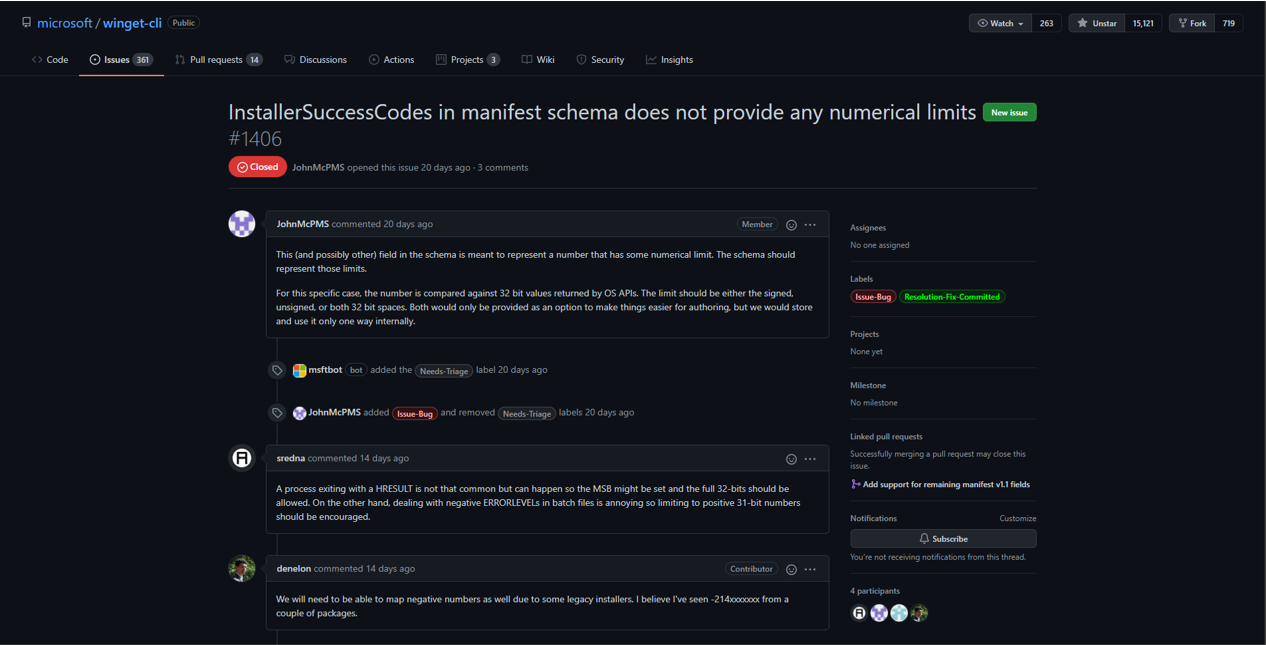
\includegraphics[width=\textwidth]{img/gh_repository_issue.png}
	\caption{Aspecto de una incidencia en GitHub.}
	\label{fig:gh_repository_issue}
\end{figure}

Las incidencias disponen de múltiples propiedades mediante las cuales detallar su finalidad, establecer su clasificación con respecto a las temáticas definidas en forma de etiquetas por el repositorio, asignar su resolución a personas concretas implicadas en el desarrollo del proyecto, gestionar su resolución y progreso en torno a hitos o versiones, comentarios realizados por el creador u otros usuarios que permiten complementar, extender o proponer resoluciones y mejoras a lo planteado inicialmente.

\subsubsection{Etiqueta} \label{sec:etiqueta}

En \emph{GitHub} una etiqueta \cite{ct:github_label} es elemento conformado por un identificador, un código de color hexadecimal y opcionalmente, una descripción que explique más en detalle la intención que señala dicho identificador. Las etiquetas son declaradas a nivel de repositorio, y pueden ser asignadas a incidencias, peticiones de cambios y discusiones. La intención de estas etiquetas consiste en establecer una clasificación de los diferentes objetos del repositorio entorno a una serie de categorías que permitan localizar de manera más rápida aquellos elementos relacionados con la temática de la etiqueta.

Por defecto en la creación de un repositorio se añaden una serie de etiquetas que posteriormente pueden ser editadas o eliminadas. Estas etiquetas base son: \emph{bug}, \emph{documentation}, \emph{duplicate}, \emph{enhancement}, \emph{good first issue}, \emph{help wanted}, \emph{invalid}, \emph{question} y \emph{wontfix} \cite{ct:github_managing_labels}.

\begin{figure}[!ht]
	\centering
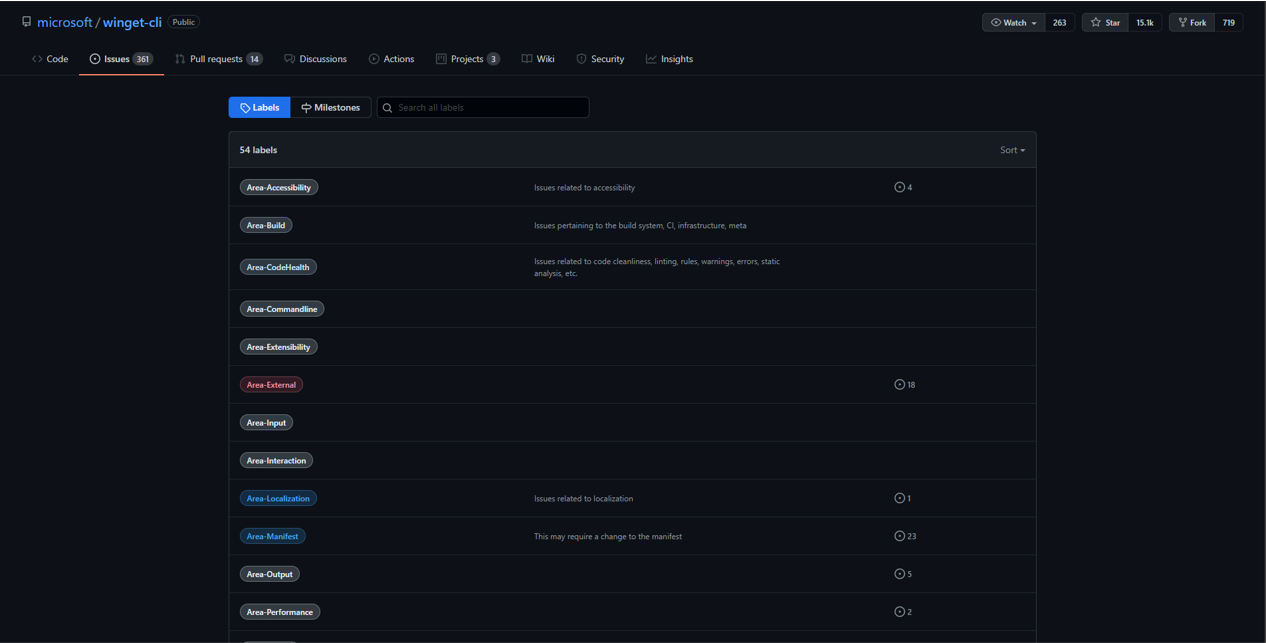
\includegraphics[width=\textwidth]{img/gh_repository_tags.png}
	\caption{Etiquetas de un repositorio en GitHub.}
	\label{fig:gh_repository_tags}
\end{figure}

\section{Conceptos teóricos relativos a la extracción y procesamiento de los datos} \label{sec:conceptosextraccionprocesamiento}

\subsection{Minería de Datos} \label{sec:mineriadatos}

La minería de datos consiste en la aplicación de técnicas de \textbf{Inteligencia Artificial (IA)} sobre grandes cantidades de datos cuyo objetivo trata de localizar patrones, tendencias o establecer relaciones entre estos. Dentro de las técnicas que componen la IA, la minería de datos se relaciona con campos de aprendizaje como el aprendizaje computacional, la estadística y las bases de datos. Este conjunto de metodologías se engloba dentro de una etapa denominada \textbf{Descubrimiento de Conocimiento en Bases de Datos (KDD)}, la cual tiene como objetivo someter a los datos a una serie de restricciones de eficiencia que dan lugar a una enumeración de los patrones localizados \cite{ct:machine_learning}.

La minería de datos permite la aplicación de multitud de técnicas para el descubrimiento de patrones en los datos. A modo de establecer una separación de acuerdo con el tipo de patrones que tratan de descubrir al aplicar dichas técnicas surgen las siguientes tres categorías principales: \hyperref[sec:mddprediccion]{predicción}, \hyperref[sec:mddanalisisasociaciones]{análisis de asociaciones} y \hyperref[sec:mddclustering]{clustering}.

\subsubsection{Predicción} \label{sec:mddprediccion}

La predicción engloba aquellas tareas que tienen como objetivo establecer relaciones entre el vector de características que conforman los elementos a clasificar y el atributo objetivo con el que se desea determinar su relación. En las tareas de predicción podemos señalar dos categorías en función del tipo de atributo objetivo que se esté prediciendo:

\vspace{-0.5cm}
\begin{itemize} [\textbullet]
	\item \textbf{Clasificación}. Las tareas de clasificación se caracterizan debido a que el atributo objetivo debe pertenecer a una clase determinada de entre un número limitado de opciones establecidas al comienzo del experimento.
	\item \textbf{Regresión}. En las tareas de regresión su principal característica se encuentra en el hecho de que el atributo objetivo debe ser de tipo numérico y su valor comprenderá un intervalo infinito de valores.
\end{itemize}

\subsubsection{Análisis de asociaciones} \label{sec:mddanalisisasociaciones}

En el análisis de asociaciones el objetivo es la revelación de hechos que suceden de manera conjunta dentro de un conjunto determinado de datos. Estos datos revelados pueden retornar cualquier atributo de los elementos implicados e incluso combinaciones entre ellos.

\subsubsection{Clustering} \label{sec:mddclustering}

El clustering comprende la aplicación de técnicas de machine learning y aprendizaje supervisado con el objetivo de identificar subconjuntos de datos con similares características entre los elementos que los componen dentro de un gran conjunto de datos.

\subsection{Recogida de los datos} \label{sec:extraccion}

La recogida de los datos la primera fase dentro de cualquier proyecto de minería de datos. Es necesario realizar un estudio previo acotando los datos que se desea conseguir y la forma en la que se va a llevar a cabo su recolección.

\begin{figure}[!ht]
	\centering
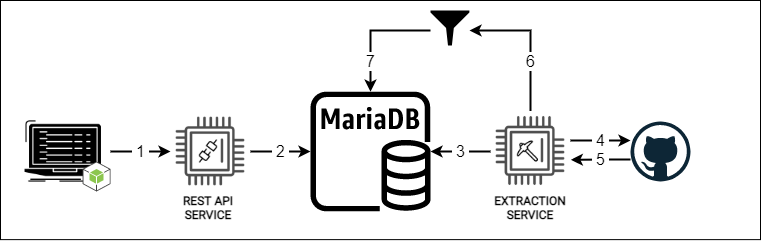
\includegraphics[width=\textwidth]{img/extraction_process.png}
	\caption{Esquema que representa el proceso seguido para la extracción de la información desde un repositorio GitHub a partir de una petición generada desde la plataforma.}
	\label{fig:extraction_process}
\end{figure}

En nuestro proyecto la extracción de los datos requiere del lanzamiento de peticiones contra la API REST de GitHub. El ámbito de la información a recoger contempla la dirección, título, descripción y etiquetas del repositorio, así como el título, autor, cuerpo, etiquetas y comentarios de las incidencias que este posea.

\subsection{Preprocesamiento de los datos} \label{sec:preprocesamiento}

Los datos en crudo extraídos por medio de la conexión con GitHub poseen impurezas que deben ser filtradas con el objetivo de almacenar la información estrictamente necesaria para la posterior aplicación de los diferentes modelos de procesamiento. Estas impurezas pueden aparecer principalmente debido al lenguaje de marcado Markdown, el cual es soportado por GitHub en el cuerpo de las incidencias y comentarios de los repositorios. Su uso está muy extendido a lo largo de los usuarios de GitHub ya que mediante la incorporación de secuencias fáciles de recordar permiten estilizar los textos de modo que al renderizarse la información facilita su lectura.

\begin{figure}[!ht]
	\centering
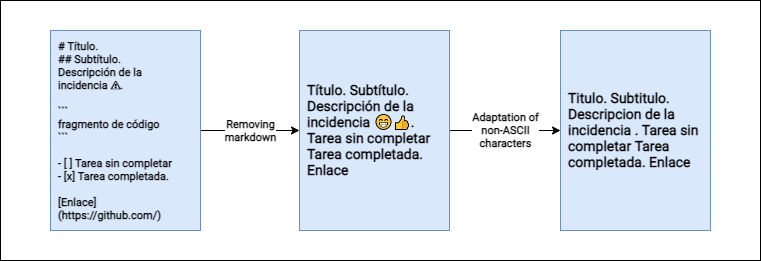
\includegraphics[width=\textwidth]{img/extraction_preprocessing_process.png}
	\caption{Esquema que representa los procesos de preprocesado a los que se somete la información extraída desde GitHub.}
	\label{fig:apply_preprocessing}
\end{figure}

Otras impurezas con las que podemos encontrarnos es con la aparición de fragmentos de código entre medias de los textos. Esta información resulta complementen irrelevante para el propósito que nos concierne y serán eliminados para evitar confundir a los modelos.

\section{Conceptos teóricos relativos al Procesamiento de los Datos} \label{sec:procesamientodatos}

\subsection{Aprendizaje profundo (Deep learning)} \label{sec:deeplearning}

El aprendizaje profundo \cite{ct:deep_learning} consiste en un conjunto de metodologías de aprendizaje automático basadas en la aplicación de redes neuronales artificiales que hacen uso del aprendizaje por representación. Este último tipo de aprendizaje por representación otorga al aprendizaje profundo una de sus principales propiedades, la simulación del comportamiento del cerebro humano. Para llevar a cabo esta compleja labor se requiere del uso de redes neuronales artificiales compuestas por multitud de capas de neuronas interconectadas, y es por ello este aprendizaje recibe el calificativo de “aprendizaje profundo”.

El proceso de entrenamiento que se sigue para este tipo de técnicas puede variar entre aprendizaje supervisado \cite{wiki:supervised_learning}, aprendizaje parcialmente supervisado \cite{wiki:semi_supervised_learning} o aprendizaje no supervisado \cite{wiki:unsupervised_learning} en función de las entradas que se dispongan y el tipo de tareas para las que se haya diseñado.

\subsection{Procesamiento del lenguaje natural (Natural lenguage processing)} \label{sec:pln}

El Procesamiento del Lenguaje Natural (PLN) \cite{ct:pln_universidad_san_marcos} es un subconjunto de técnicas de aprendizaje profundo cuyos métodos tratan de generar modelos de inteligencia artifical (IA) enfocados en el estudio y comprensión de los mecanismos que conforman el lenguaje humano de manera que posteriormente sean capaces de reproducir estos comportamientos. En los últimos años los sistemas basados en el PLN han adquirido una importante popularidad debido a la amplia variedad de tareas cuyos comportamientos son aplicables. Entre sus aplicaciones más destacables se encuentran: la \hyperref[sec:summarization]{generación de resúmenes}, la \hyperref[sec:clasificadorzeroshot]{clasificación de textos}, la traducción, el \hyperref[sec:analisissentimientos]{análisis de sentimientos} y los agentes conversacionales.

\subsection{Modelos preentrenados aplicados al PLN} \label{sec:preentrenados}

Los modelos de PLN requieren de un exhaustivo entrenamiento previo a su puesta en marcha con el objetivo de lograr obtener unos buenos resultados. Para ello se precisa de grandes conjuntos de datos previamente depurados para permitir al modelo establecer relaciones entre los datos y asimilar los patrones localizados.

\begin{figure}[!ht]
	\centering
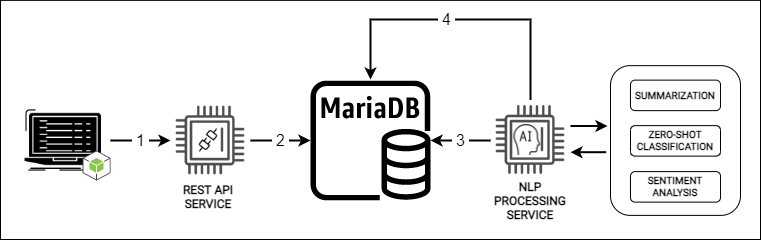
\includegraphics[width=\textwidth]{img/applying_nlp_process.png}
	\caption{Esquema que representa el proceso seguido para aplicación de los modelos de PLN a partir de una petición generada desde la plataforma.}
	\label{fig:apply_nlp_process}
\end{figure}

Los modelos preentrenados \cite{ct:pretrained_models} son una nueva tendencia que trata de minimizar los recursos invertidos en la construcción desde cero de este tipo de modelos. Su fundamento consiste en proporcionar modelos de propósito general entrenados a partir de grandes \emph{datasets} con la premisa de proporcionar una base funcional a los desarrolladores de este tipo de proyectos. El inconveniente de este tipo de modelos se encuentra en la pérdida de precisión en campos de aplicación específicos, aunque estos efectos siempre pueden mitigarse a través de la introducción de ajustes en los parámetros de configuración del modelo.

\subsubsection{Zero Shot Classification} \label{sec:clasificadorzeroshot}

El modelo preentrenado <<\textbf{bart-large-mnli}>> \cite{huggingface:bart_large_mnli} diseñado por la división de Inteligencia Artificial de \emph{Facebook} es el escogido para la aplicación del procesado utilizando la técnica de \emph{Zero-Shot Classification}. Este modelo ha sido entrenado haciendo uso del \emph{dataset} \textbf{MultiNLI} y está basado en el modelo preentrenado \textbf{Bidirectional and Auto-Regressive Transformer (BART)}.

El modelo se basa en la tecnología de modelos \textbf{Inferencia del Lenguaje Natural (NLI)}, un subconjunto de los modelos de Procesamiento del Lenguaje Natural (PLN), los cuales tratan de determinar si una hipótesis es verdadera, falsa o neutral a partir de una premisa dada. Estos sistemas son entrenados a partir de grandes \emph{datasets} que contienen una serie de premisas, una hipótesis por cada premisa y una etiqueta que identifica la relación entre ambas.

El funcionamiento del concreto de este modelo consiste en la \textbf{generación de hipótesis} a partir de la secuencia a analizar y cada una de las etiquetas introducida. Una vez se construyen las hipótesis estas son evaluadas de acuerdo con sus \textbf{índices de implicación y contradicción} obteniendo un valor para cada hipótesis. Estos valores serán los asignados a las etiquetas como probabilidad de que exista una relación entre la cadena introducida y la etiqueta.

\subsubsection{Sentiment Analysis} \label{sec:analisissentimientos}

La elección de una implementación para la aplicación de \emph{Sentiment Analysis} \cite{huggingface:bert_base_multilingual_uncased_sentiment}es el modelo preentrenado <<\textbf{bert-base-multilingual-uncased-sentiment}>> desarrollado por \emph{NLP Town} partiendo como base del modelo \textbf{Bidirectional Encoder Representations from Transformers (BERT)}. Esta implementación en concreto ha sido entrenada con más de 620k reseñas de productos en seis idiomas distintos: inglés, francés, alemán, holandés, italiano y español.

Su funcionamiento trata de predecir el \textbf{grado de satisfacción} de la secuencia introducida otorgándole una puntuación \textbf{entre 1 y 5 estrellas}. Según las pruebas a las que ha sido sometido este modelo, la precisión con la que es capaz de predecir la puntuación otorgada de manera exacta es de media un \textbf{60\%}, que se amplía hasta un \textbf{94\%} en el caso de predicciones con una desviación de un nivel por encima o por debajo de la valoración original. Además de retornar la puntuación en estrellas, este modelo es capaz de retornar la puntuación exacta calculada, que es el valor que utilizaremos en nuestro caso para reflejar los resultados obtenidos.

\subsubsection{Summarization} \label{sec:summarization}

En el caso de la tarea de \emph{Summarization} \cite{huggingface:distilbart_cnn_12_6} el modelo preentrenado utilizado es el <<\textbf{distilbart-cnn-12-6}>> creado por \emph{Sshleifer}. Este modelo se basa en una versión reducida del modelo \emph{BART} denominada \textbf{DistilBART} que reduce los tiempos de generación a costa de una pequeña pérdida de rendimiento.

Existen dos tipos de técnicas utilizadas en la generación de resúmenes:

\begin{itemize} [\textbullet]
    \item \textbf{Generación de resúmenes por extracción}. La generación de resúmenes extractivos tiene como objetivo la obtención de resúmenes a partir de \textbf{fragmentos extraídos del texto original}. Para llevar a cabo este proceso, el modelo se encarga de puntuar las diferentes oraciones que componen el enunciado introducido de acuerdo a una predicción de la importancia que tiene su contenido sobre el global de la información original. A partir de este \emph{ranking} el modelo escoge los enunciados de mayor puntuación con la finalidad de que el texto obtenido condense las principales ideas del enunciado original.
    
    \item \textbf{Generación de resúmenes por abstracción}. La generación de resúmenes por medio de técnicas de abstracción tiene como objetivo la generación de \textbf{nuevo contenido} a partir de las ideas del texto original. El proceso de generación de este tipo de resúmenes inicialmente se encarga de mezclar las oraciones del enunciado introducido. El siguiente paso consisten en reemplazar ciertos fragmentos del texto por máscaras. Por último, estas máscaras son reemplazadas por un pequeño conjunto de palabras, una palabra o un símbolo de puntuación.
\end{itemize}

El modelo escogido tiene como propósito la generación de resúmenes abstractivos adecuándose a los parámetros de longitud mínima y máxima establecidos. El entrenamiento del modelo fue llevado a cabo haciendo uso del \emph{dataset} de \textbf{cnn\_dailymail} \cite{ct:dailymail}, el cual contiene numerosos artículos periodísticos que son tratados como entrada, y una serie de ideas clave del artículo que se unen formando el texto objetivo que se pretende alcanzar.
